\section{Speicher - Lukas}
\subsection{Typen von Speicher in FPGA}
In einem FPGA sind normalerweise zwei Arten von Speicher vorhanden:
\begin{compactitem}
    \item \textbf{Distributed Memory}: Distributed Memory besteht aus vielen LUT Tabellen. Der Vorteil dieser Variante ist, dass jede beliebige Grösse von Speicher realisiert werden kann. Desweitern kann dieser Speicher an jedem Ort in einem FPGA erstellt werden. Ideal für kleine Speichergrössen.
    \item \textbf{Block Memory}: Block Memory sind fest implementierte Speicherzellen (Hard IP Block). Diese bestehen aus SRAM Zellen (zwei kreuzgekoppelte Inverter) und sind über das ganze FPGA hinweg verteilt. Oftmals haben sie auch gerade eine Fehlerkorrektur implementiert (bei Xilinx: Hamming Error Correction Code). Ideal für grössere Speichergrössen. Die Speichergrösse bei den Xilinx Series 7 Block Rams beträgt 32kb (36kb physikalisch vorhanden).
\end{compactitem}

\subsubsection{ROM}
ROM wird benutzt um konstante Daten zu speichern. In einem FPGA wird die Implementierung von ROM mithilfe von RAM gemacht.

\subsubsection{Interface Arten}
Beide Speicherarten können mit zwei verschiedenen Schnittstellen implementiert werden.

\begin{minipage}{0.3\textwidth}
    \begin{figure}[H]
        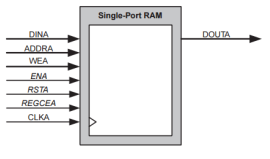
\includegraphics[width=1\textwidth]{images/singleportram.png}
    \end{figure}
\end{minipage}
\hfill
\begin{minipage}{0.65\textwidth}
    \paragraph{Single-Port RAM}
    Single-Port RAM hat einen Daten und einen Adressbus. Darüber sind sequentielle Lese- und Schreibzugriffe möglich. Wird Distributed Memory verwendet, so ist es auch zusätzlich noch möglich asynchrone Lesezugriffe durchzuführen. \ \\ \ \\ \ \\
\end{minipage}

\begin{minipage}{0.3\textwidth}
    \begin{figure}[H]
        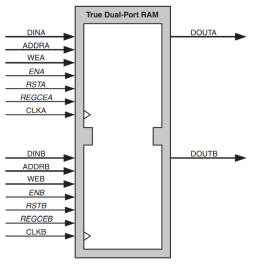
\includegraphics[width=1\textwidth]{images/dualportram.png}
    \end{figure}
\end{minipage}
\hfill
\begin{minipage}{0.65\textwidth}
    \paragraph{Dual-Port RAM}
    Dual-Port RAM erlaubt zwei gleichzeitige Lese- und/oder Schreibzugriffe. Wird über beide Schnittstellen auf die gleiche Speicherzelle zugegriffen, so gibt es eine Arbitrierschaltung, welche diese Situation korrekt abwickelt. \ \\ \ \\ \ \\ \ \\ \ \\ \ \\ \ \\ \ \\ \ \\ \ \\
\end{minipage}


\subsection{Beschreibung von Speicher in VHDL}
Es existieren vier Richtlinien für das Beschreiben von ROM und RAM in VHDL. Wird Speicher anhand dieser Richtlinien beschrieben, so sollte der Synthesizer den Speicher korrekt implementieren.
\begin{compactenum}
    \item Die Datengrösse und die Adressengrösse soll mit generischen Parametern definiert werden.
    \item Der Addressenbereich soll mit einer Konstante definiert werden.
    \item RAM soll mit einem zweidimensionalen Array beschrieben werden.
    \item Der Schreibzugriff muss in einem Prozess beschrieben werden.
\end{compactenum}

\subsubsection{Block RAM - Single-Port}
\lstinputlisting[language=VHDL]{code/blockram_single.vhd}

\subsubsection{Distributed RAM - Single-Port}
\lstinputlisting[language=VHDL]{code/distributedram_single.vhd}

\subsubsection{Block RAM - Dual-Port}
\lstinputlisting[language=VHDL]{code/blockram_dual.vhd}

\subsubsection{ROM}
Da ROM gleich wie RAM implementiert wird, muss nur das RAM Signal als Konstante definiert werden.
\lstinputlisting[language=VHDL]{code/rom.vhd}

\subsubsection{Synthese Attribut}
Mit dem Attribut \texttt{ram\_style} kann Vivado mitgeteilt werden ob das RAM als Distributed RAM (\texttt{"distributed"}) oder als Block RAM (\texttt{"block"}) implementiert werden soll.
\lstinputlisting[language=VHDL]{code/ram_attribute.vhd}

\subsubsection{Initialisierung}
Eine einfache Art um Speicher zu initialisieren, kann mit Hilfe einer Funktion und einer Datei erreicht werden.
\lstinputlisting[language=VHDL]{code/ram_init.vhd}

Der Speicher kann aber auch direkt im Code initialisiert werden (eher aufwändig und unübersichtlich):
\lstinputlisting[language=VHDL]{code/ram_init2.vhd}

\subsection{Memory IP Generators}
Vivado stellt verschiedene IP Generatoren zur Verfügung, über welche direkt Speicher instantiiert werden kann. Diese Generatoren stellen eine einfache Möglichkeit um Speicher nach den eigenen Wünschen zu konfigurieren. Ebenfalls stellen sie präzise Simulationsmodelle zur Verfügung.